\section{Практика 3 (Аналіз системи)}

$\ddot{x} + 2\gamma\dot{x} +\omega_0^2x = 0$

Складемо систему

\begin{minipage}{0.40\textwidth}
    $\left\{\begin{aligned}
        \frac{dy}{dt} &= -2\gamma y - \omega_0^2x \\
        \frac{dx}{dt} &= y
    \end{aligned}\right.$
    \\[2mm]
    $\overrightarrow{u} = \begin{bmatrix} y\\x \end{bmatrix} \ \ 
    A = \begin{bmatrix}
        -2\gamma & -\omega_0^2 \\
        1 & 0
    \end{bmatrix}$ 
\end{minipage}
\begin{minipage}{0.49\textwidth}
    $\gamma \ge 0, \ \omega_0 \ge 0$\\[2mm]
    $\overrightarrow{u}$ --- вектор стану\\
    $\overrightarrow{b} $ --- власний вектор матриці $A$\\
    $\lambda_i$ --- власні числа матриці $A$\\[1mm]
\end{minipage}

\begin{equation}\label{pr3:eq1}
    \frac{d\overrightarrow{u}}{dt} = A\overrightarrow{u}
\end{equation}


Шукаємо розвязок (\ref{pr3:eq1}) у вигляді $\overrightarrow{u} = \overrightarrow{b}e^{\lambda t}$

\subsection{Завдання 1: (Знайти власні числа)}

$\det (A - \lambda E) = 0$

$\begin{vmatrix}
    -2\gamma  - \lambda & -\omega_0^2 \\
        1 & -\lambda
\end{vmatrix} = \lambda^2 + 2\gamma\lambda + \omega_0^2 = 0$  розв'язавши отримуємо власні числа


\begin{equation}\label{pr3:eigenval}
    \lambda_{1,2} = - \gamma \pm \sqrt{\gamma^2 - \omega^2_0}
\end{equation}



\subsection{Завдання 2: (Знайти власні вектора)}

$(A - \lambda E)\overrightarrow{b}  = 0$

$\begin{bmatrix}
    -2\gamma  - \lambda & -\omega_0^2 \\
        1 & -\lambda
\end{bmatrix} \begin{bmatrix}
    b_1 \\ b_2
\end{bmatrix}  = 0$

\begin{numcases}{}
    (-2\gamma  - \lambda)b_1  -\omega_0^2 b_2 = 0 \label{pr3:eq2}
    \\
    b_1  - \lambda b_2 = 0 \label{pr3:eq3}
\end{numcases}

Із рівності (\ref{pr3:eq3}) отримуємо, що $\frac{b_1}{b_2} = \lambda$, тоді 
власними векторами будуть 
\begin{equation}\label{pr3:eigenvec}
    \overrightarrow{b^1} = c_1 \begin{bmatrix}
        \lambda_1 \\ 1
    \end{bmatrix} \ \ 
    \overrightarrow{b^2} = c_2 \begin{bmatrix}
        \lambda_2 \\ 1
    \end{bmatrix}, \ c_1, c_2 \in \mathbb{R} 
\end{equation}



\subsection{Завдання 3: (Знайти розв'язок системи)}

Розв'язком системи (\ref{pr3:eq1}) буде 

$$
    \begin{bmatrix}
        u_1 \\ u_2
    \end{bmatrix} = 
    c_1 \begin{bmatrix}
        \lambda_1 \\1
    \end{bmatrix} e^{\lambda_1 t} + 
    c_2 \begin{bmatrix}
        \lambda_2 \\1
    \end{bmatrix} e^{\lambda_2 t} = \Bigg(
    c_1 \begin{bmatrix}
        \lambda_1 \\1
    \end{bmatrix} e^{t\sqrt{\gamma^2 - \omega_0^2}} + 
    c_2 \begin{bmatrix}
        \lambda_2 \\1
    \end{bmatrix} e^{-t\sqrt{\gamma^2 - \omega_0^2}} \Bigg) e^{-\gamma t}
$$

позначимо $\omega^2 = \omega_0^2 - \gamma^2$, тоді отримаємо систему

\begin{equation}\label{pr3:solution}
    \begin{bmatrix}
        u_1 \\ u_2
    \end{bmatrix} =  \Bigg(
    c_1 \begin{bmatrix}
        \lambda_1 \\1
    \end{bmatrix} e^{i\omega t} + 
    c_2 \begin{bmatrix}
        \lambda_2 \\1
    \end{bmatrix} e^{-i\omega t} \Bigg) e^{-\gamma t}
\end{equation}



якби для пошуку власних векторів сористались не рівністю (\ref{pr3:eq3}), а рівністю
(\ref{pr3:eq2}), отримали б рішення

$$
\begin{bmatrix}
    u_1 \\ u_2
\end{bmatrix} =  \Bigg(
c_1^* \begin{bmatrix}
    -\omega_0 \\ \lambda_1 + \gamma
\end{bmatrix} e^{i\omega t} + 
c_2^* \begin{bmatrix}
    -\omega_0 \\\lambda_2 + \gamma
\end{bmatrix} e^{-i\omega t} \Bigg) e^{-\gamma t}
$$

\subsection{Завдання 4: (Знайти траєкторію)}

$\left\{\begin{aligned}
    \frac{dy}{dt} &= -2\gamma y - \omega_0^2x \\
    \frac{dx}{dt} &= y
\end{aligned}\right.$

$\frac{dy}{dx} = -2\gamma - \omega^2_0 \frac{x}{y} \ \ \Bigg | \ y = xz, \ dy = zdx + xdz$

$z + x\frac{dz}{dx} = -2\gamma - \frac{\omega_0^2}{z}$

$-\frac{dx}{x} = \frac{dz}{z + 2\gamma + \frac{\omega_0^2}{z}} \ \ \Bigg | \cdot \frac{z}{z}$

$-\frac{dx}{x} = \frac{zdz}{z^2 + 2\gamma z + \omega_0^2} = 
\frac{zdz}{(z^2 + 2\gamma z + \gamma ^2) - (\gamma^2 - \omega_0^2)} \ \ \Bigg | \Delta =  \gamma^2 - \omega_0^2$

$-\frac{dx}{x} = \frac{zdz}{(z + \gamma)^2 - \Delta} = 
\frac{(z + \gamma - \gamma)d(z+\gamma)}{(z + \gamma)^2 - \Delta} = 
\frac{(z + \gamma)d(z+\gamma)}{(z + \gamma)^2 - \Delta} - \gamma\frac{d(z+\gamma)}{(z + \gamma)^2 - \Delta}$

$-\frac{dx}{x} = \frac{1}{2}\frac{d((z+\gamma)^2 - \Delta)}{(z + \gamma)^2 - \Delta} - \gamma\frac{d(z+\gamma)}{(z + \gamma)^2 - \Delta}$

\begin{equation} \label{pr3:eq8}
    -\ln x = \frac{1}{2} \ln {((z+\gamma)^2 - \Delta)} - \gamma \int \frac{d(z+\gamma)}{(z + \gamma)^2 - \Delta} + \ln C_0
\end{equation}


% $\Bigg [ \frac{d(z+\gamma)}{(z + \gamma)^2 - \Delta}  = \Big | p = z + \gamma, \ dp = d(z+\gamma) \ \Big | = 
% \frac{dp}{p^2 - \Delta} = \frac{dp}{(p + \sqrt{\Delta})(p - \sqrt{\Delta})}  = 
% \Big [ \frac{A}{p + \sqrt{\Delta}} + \frac{B}{p - \sqrt{\Delta}} = \frac{Ap - A\sqrt{\Delta} + Bp + B\sqrt{\Delta}}{(p + \sqrt{\Delta})(p - \sqrt{\Delta})}  =\\
%  = \left\{\begin{aligned}
%     B - A = 1\\
%     B + A = 0
% \end{aligned}\right. \Longrightarrow \ B = \frac{1}{2}, \ \ A = -\frac{1}{2} \Big ] = 
% \frac{1}{2} \Big (\frac{dp}{p + \sqrt{\Delta}} - \frac{dp}{p - \sqrt{\Delta}}\Big) = \frac{1}{2}\Big(\frac{d(z-\gamma)}{(z-\gamma) + \sqrt{\Delta}} - \frac{d(z-\gamma)}{(z-\gamma) - \sqrt{\Delta}}\Big) \Bigg ]$


% отже рівність (\ref{pr3:eq8}) приймає вигляд 

% $\ln x^2 + \ln {((z+\gamma)^2 - \Delta)} = \gamma \ln\frac{(z+\gamma) + \sqrt{\Delta}}{(z+\gamma) - \sqrt{\Delta}} + C_1$

Нехай $\Delta < 0$ тоді  (\ref{pr3:eq8}) матиме вигляд 

$-\ln x = \frac{1}{2} \ln {((z+\gamma)^2 + |\Delta|)} - \gamma \int \frac{d(z+\gamma)}{(z + \gamma)^2 + |\Delta|} + \ln C_0$

$-\ln x = \frac{1}{2} \ln {((z+\gamma)^2 + \Delta)} - \frac{\gamma}{\sqrt{|\Delta|}} \arctg \frac{z+\gamma}{\sqrt{|\Delta|}}+ \ln C$

$\ln x^2((z+\gamma)^2 +|\Delta|) = \frac{2\gamma}{\sqrt{|\Delta|}} \arctg \frac{z+\gamma}{\sqrt{|\Delta|}} - \ln C^2$

$\ln ( x^2z^2+x^2\gamma z + \gamma^2 - \gamma^2 + \omega_0^2) = \frac{2\gamma}{\omega} \arctg \frac{z+\gamma}{\omega} - \ln C^2$

\begin{equation}
    \ln ( y^2+\gamma xy + \omega_0^2 x^2) = \frac{2\gamma}{\omega} \arctg \frac{y+\gamma x}{\omega x} - \ln C^2
\end{equation}

% Нехай $\Delta > 0, \gamma > \omega_0$ тоді  (\ref{pr3:eq8}) матиме вигляд

% $-\frac{dx}{x} = \frac{zdz}{z^2 + 2\gamma z + \omega_0^2} = 
% \frac{zdz}{(z-(-\gamma+\sqrt{\Delta}))(z-(-\gamma-\sqrt{\Delta}))} = 
% \frac{zdz}{(z-\lambda_1)(z-\lambda_2)} = \Big| \frac{A}{z-\lambda_1} + \frac{B}{z-\lambda_2} \Longrightarrow\\ \Longrightarrow
% \left\{\begin{aligned}
%     &\lambda_2 A + \lambda_1 B = 0\\
%     &A + B = 1
% \end{aligned}\right. \Longrightarrow 
% \left\{\begin{aligned}
%     &\lambda_2 (1-B) + \lambda_1 B = 0\\
%     &A = 1 - B
% \end{aligned}\right. \Longrightarrow 
% \left\{\begin{aligned}
%     A = \frac{-\lambda_1}{\lambda_2 - \lambda_1}\\
%     B = \frac{\lambda_2}{\lambda_2 - \lambda_1}
% \end{aligned}\right| \Longrightarrow \\ \Longrightarrow
% -\frac{dx}{x} =  \frac{\lambda_2}{\lambda_2 - \lambda_1}\frac{dz}{z-\lambda_2} - 
% \frac{\lambda_1}{\lambda_2 - \lambda_1} \frac{dz}{z-\lambda_1}$

% $\ln|x| =  -\frac{\lambda_2}{\lambda_2 - \lambda_1}\ln|z-\lambda_2| + 
% \frac{\lambda_1}{\lambda_2 - \lambda_1} \ln|z-\lambda_1|$

\subsection{Завдання 5:}

$\ddot{x} + 2\gamma\dot{x}+\omega_0^2x = 0 \ \Longrightarrow \ 
\left\{\begin{aligned}
    \frac{dy}{dt} &= -2\gamma y -\omega_0^2x\\
    \frac{dx}{dt} &= y 
\end{aligned}\right.$

\begin{figure}[h]
    \begin{minipage}[h]{0.49\linewidth}
        %% Creator: Inkscape 1.0 (4035a4f, 2020-05-01), www.inkscape.org
%% PDF/EPS/PS + LaTeX output extension by Johan Engelen, 2010
%% Accompanies image file 'pr1_4.pdf' (pdf, eps, ps)
%%
%% To include the image in your LaTeX document, write
%%   \input{<filename>.pdf_tex}
%%  instead of
%%   \includegraphics{<filename>.pdf}
%% To scale the image, write
%%   \def\svgwidth{<desired width>}
%%   \input{<filename>.pdf_tex}
%%  instead of
%%   \includegraphics[width=<desired width>]{<filename>.pdf}
%%
%% Images with a different path to the parent latex file can
%% be accessed with the `import' package (which may need to be
%% installed) using
%%   \usepackage{import}
%% in the preamble, and then including the image with
%%   \import{<path to file>}{<filename>.pdf_tex}
%% Alternatively, one can specify
%%   \graphicspath{{<path to file>/}}
%% 
%% For more information, please see info/svg-inkscape on CTAN:
%%   http://tug.ctan.org/tex-archive/info/svg-inkscape
%%
\begingroup%
  \makeatletter%
  \providecommand\color[2][]{%
    \errmessage{(Inkscape) Color is used for the text in Inkscape, but the package 'color.sty' is not loaded}%
    \renewcommand\color[2][]{}%
  }%
  \providecommand\transparent[1]{%
    \errmessage{(Inkscape) Transparency is used (non-zero) for the text in Inkscape, but the package 'transparent.sty' is not loaded}%
    \renewcommand\transparent[1]{}%
  }%
  \providecommand\rotatebox[2]{#2}%
  \newcommand*\fsize{\dimexpr\f@size pt\relax}%
  \newcommand*\lineheight[1]{\fontsize{\fsize}{#1\fsize}\selectfont}%
  \ifx\svgwidth\undefined%
    \setlength{\unitlength}{289.26128237bp}%
    \ifx\svgscale\undefined%
      \relax%
    \else%
      \setlength{\unitlength}{\unitlength * \real{\svgscale}}%
    \fi%
  \else%
    \setlength{\unitlength}{\svgwidth}%
  \fi%
  \global\let\svgwidth\undefined%
  \global\let\svgscale\undefined%
  \makeatother%
  \resizebox*{\sz}{\sz}{%
  \begin{picture}(1,1)%
    \lineheight{1}%
    \setlength\tabcolsep{0pt}%
    \put(0,0){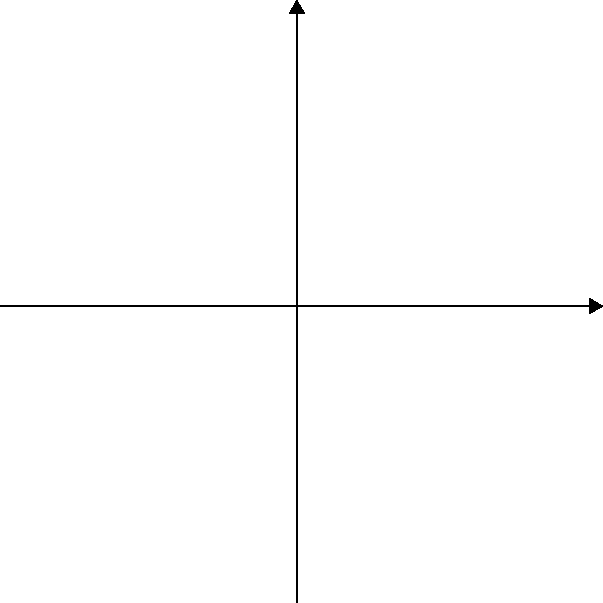
\includegraphics[width=\unitlength,page=1]{practices/1_pr/source/pr1_4.pdf}}%
    \put(0.42420684,0.92372983){\color[rgb]{0,0,0}\makebox(0,0)[lt]{\lineheight{1.25}\smash{\begin{tabular}[t]{l}$Y$\end{tabular}}}}%
    \put(0.8969896,0.43585215){\color[rgb]{0,0,0}\makebox(0,0)[lt]{\lineheight{1.25}\smash{\begin{tabular}[t]{l}$X$\end{tabular}}}}%
    \put(0,0){\includegraphics[width=\unitlength,page=2]{practices/1_pr/source/pr1_4.pdf}}%
  \end{picture}%
  }
\endgroup%
 \\
        \centering {a)}
    \end{minipage}
    \begin{minipage}[h]{0.49\linewidth}
        %% Creator: Inkscape 1.0 (4035a4f, 2020-05-01), www.inkscape.org
%% PDF/EPS/PS + LaTeX output extension by Johan Engelen, 2010
%% Accompanies image file 'pr1_5.pdf' (pdf, eps, ps)
%%
%% To include the image in your LaTeX document, write
%%   \input{<filename>.pdf_tex}
%%  instead of
%%   \includegraphics{<filename>.pdf}
%% To scale the image, write
%%   \def\svgwidth{<desired width>}
%%   \input{<filename>.pdf_tex}
%%  instead of
%%   \includegraphics[width=<desired width>]{<filename>.pdf}
%%
%% Images with a different path to the parent latex file can
%% be accessed with the `import' package (which may need to be
%% installed) using
%%   \usepackage{import}
%% in the preamble, and then including the image with
%%   \import{<path to file>}{<filename>.pdf_tex}
%% Alternatively, one can specify
%%   \graphicspath{{<path to file>/}}
%% 
%% For more information, please see info/svg-inkscape on CTAN:
%%   http://tug.ctan.org/tex-archive/info/svg-inkscape
%%
\begingroup%
  \makeatletter%
  \providecommand\color[2][]{%
    \errmessage{(Inkscape) Color is used for the text in Inkscape, but the package 'color.sty' is not loaded}%
    \renewcommand\color[2][]{}%
  }%
  \providecommand\transparent[1]{%
    \errmessage{(Inkscape) Transparency is used (non-zero) for the text in Inkscape, but the package 'transparent.sty' is not loaded}%
    \renewcommand\transparent[1]{}%
  }%
  \providecommand\rotatebox[2]{#2}%
  \newcommand*\fsize{\dimexpr\f@size pt\relax}%
  \newcommand*\lineheight[1]{\fontsize{\fsize}{#1\fsize}\selectfont}%
  \ifx\svgwidth\undefined%
    \setlength{\unitlength}{308.51451964bp}%
    \ifx\svgscale\undefined%
      \relax%
    \else%
      \setlength{\unitlength}{\unitlength * \real{\svgscale}}%
    \fi%
  \else%
    \setlength{\unitlength}{\svgwidth}%
  \fi%
  \global\let\svgwidth\undefined%
  \global\let\svgscale\undefined%
  \makeatother%
  \resizebox*{\sz}{\sz}{%
  \begin{picture}(1,0.93759374)%
    \lineheight{1}%
    \setlength\tabcolsep{0pt}%
    \put(0,0){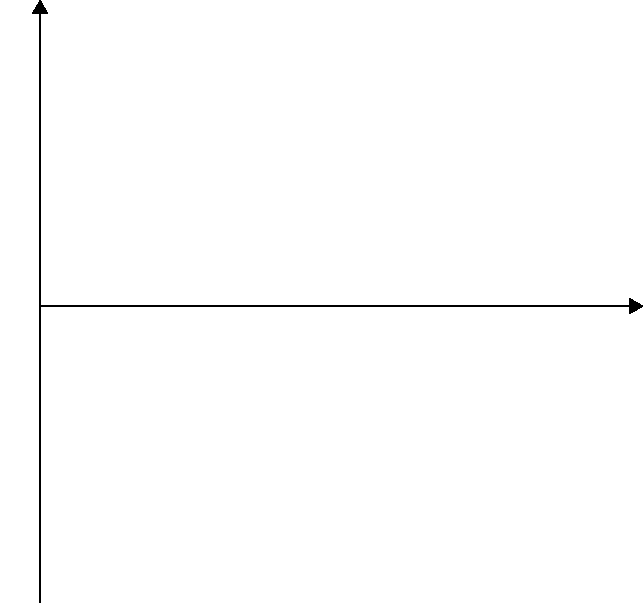
\includegraphics[width=\unitlength,page=1]{practices/1_pr/source/pr1_5.pdf}}%
    \put(-0.00177265,0.8660833){\color[rgb]{0,0,0}\makebox(0,0)[lt]{\lineheight{1.25}\smash{\begin{tabular}[t]{l}$X$\end{tabular}}}}%
    \put(0.88827117,0.37676012){\color[rgb]{0,0,0}\makebox(0,0)[lt]{\lineheight{1.25}\smash{\begin{tabular}[t]{l}$t$\end{tabular}}}}%
    \put(0,0){\includegraphics[width=\unitlength,page=2]{practices/1_pr/source/pr1_5.pdf}}%
  \end{picture}%
  }
\endgroup%
 \\
        \centering{b)}
    \end{minipage}
\end{figure}

\textbf{Знайти $\Gamma$}

$\dive \overrightarrow{V} = -2\gamma$

$\ln \Gamma = -2\gamma t + C$

$\Gamma(t) = \Gamma(0)e^{-2\gamma t}$

\textbf{Записати в полярних координатах}

$\left\{\begin{aligned}
    \frac{dy}{dt} &= -2\gamma y -\omega_0^2x\\
    \frac{dx}{dt} &= y 
\end{aligned}\right.$

$\left\{\begin{aligned}
    x = r\cos \varphi \\
    y = r\sin \varphi 
\end{aligned}\right.$

$\left\{\begin{aligned}
    \dot{r}\sin \varphi + \dot{\varphi}r \cos \varphi &=  -2\gamma r\sin \varphi - \omega_0^2 r\cos \varphi\\
    \dot{r}\cos \varphi - \dot{\varphi} r \sin \varphi &= r \sin \varphi
\end{aligned}\right.$

$\left\{\begin{aligned}
    -\dot{r} &= \dot{\varphi}r\ctg \varphi + 2\gamma r + \omega_0^2 r \ctg \varphi \\
    \dot{\varphi} &= \frac{\dot{r}\ctg \varphi }{r} - 1
\end{aligned}\right.$

$-\dot{\varphi} = \dot{\varphi} \ctg^2 \varphi + 2\gamma\ctg \varphi + \omega_0^2 \ctg^2 \varphi + 1$

$-\dot{\varphi}(1 + \ctg^2\varphi) =  2\gamma\ctg \varphi + \omega_0^2 \ctg^2\varphi + 1\ | \ 1+\ctg^2\varphi = \frac{1}{\sin^2\varphi}$ 

$\dot{\varphi} = -2\gamma\cos\varphi\sin\varphi - \omega^2_0\cos^2\varphi - \sin^2\varphi= 
-\gamma\sin 2\varphi - \omega_0^2\cos^2\varphi - \sin^2\varphi \ldots$

